%!TEX program = xelatex
\documentclass[UTF8,aspectratio=43,10pt,t]{ctexbeamer}

\mode<presentation> {
\usetheme{Madrid}
\setbeamertemplate{footline}[frame number] %设置页码
\setbeamercolor{page number in head/foot}{fg=blue} %设置页码颜色
\setbeamertemplate{navigation symbols}{} %去除控件
}
\usepackage{indentfirst}
\setlength{\parindent}{2em}
\usepackage{listings}
\usepackage{wrapfig}
\usepackage{graphicx}
%设置图片存放路径
\graphicspath{{figures/}}
\usepackage{multicol} %多列布局

%用户自定义区块环境
\usepackage{setspace}
\definecolor{hanblue}{rgb}{0.27, 0.42, 0.81}
\definecolor{indiagreen}{rgb}{0.07, 0.53, 0.03}
\definecolor{indianred}{rgb}{0.8, 0.36, 0.36}
\definecolor{indianyellow}{rgb}{0.89, 0.66, 0.34}
\definecolor{babypink}{rgb}{0.96, 0.76, 0.76}
\definecolor{ao(english)}{rgb}{0.0, 0.5, 0.0}
% \setbeamerfont{block title}{size=\small}
% \setbeamerfont{block body}{size=\small}
\setbeamerfont{block title}{}
\setbeamerfont{block body}{}
\newenvironment<>{blueblock}[1]{
    \setbeamercolor{block title}{fg=white,bg=hanblue}
    \begin{block}#2{#1}}{\end{block}}
\newenvironment<>{greenblock}[1]{
    \setstretch{1.3}\setbeamercolor{block title}{fg=white,bg=indiagreen}
    \begin{block}#2{#1}}{\end{block}}
\newenvironment<>{redblock}[1]{
    \setstretch{1.3}\setbeamercolor{block title}{fg=white,bg=indianred}
    \begin{block}#2{#1}}{\end{block}}
\newenvironment<>{yellowblock}[1]{
    \setstretch{1.3}\setbeamercolor{block title}{fg=white,bg=indianyellow}
    \begin{block}#2{#1}}{\end{block}}

\lstset{language=C++,
columns=flexible,
basicstyle=\footnotesize\ttfamily,                                      % 设定代码字体、大小
%numbers=left,xleftmargin=2em,framexleftmargin=2em,                   % 在左侧显示行号
%numberstyle=\color{darkgray},                                        % 设定行号格式
keywordstyle=\color{blue},                                            % 设定关键字格式
commentstyle=\color{ao(english)},                                     % 设置代码注释的格式
stringstyle=\color{brown},                                            % 设置字符串格式
%showstringspaces=false,                                              % 控制是否显示空格
%frame=lines,                                                         % 控制外框
breaklines,                                                           % 控制是否折行
postbreak=\space,                                                     % 控制折行后显示的标识字符
breakindent=5pt,                                                      % 控制折行后缩进数量
emph={size\_t,array,deque,list,map,queue,set,stack,vector,string,pair,tuple}, % 非内置类型
emphstyle={\color{teal}},
escapeinside={(*@}{@*)},
}

\title[\textit{C++程序设计:第十二章}]{第十二章~工具与技术}

% \author
%     []
%     {}

\date{}

% \institute
%     {}


\begin{document}

\maketitle

\begin{frame}
    {目录}
    \begin{multicols*}{2}
        \tableofcontents
    \end{multicols*}
\end{frame}

\begin{frame} {前言}
    \begin{yellowblock}{学习目标}
        \begin{enumerate}
            \item 理解并掌握命名空间的使用方法;
            \item 掌握异常处理的使用方法;
            \item 理解和使用多重继承以及虚继承;
            \item 了解嵌套类和运行时类型识别的使用方法;
            \item 学会使用标准库中一些特殊工具,包括tuple类型、bitset类型以及对日期和时间的处理。
        \end{enumerate}
    \end{yellowblock}
\end{frame}

\section{命名空间}
\begin{frame}[fragile]{12.1~命名空间}
    将大量由于共同开发等原因使用的全局名字引入到同一作用域时,不可避免会产生命名冲突,例如:
    \begin{columns}[T]
        \column{0.65\textwidth}
        \begin{blueblock}{定义相同名称的不同函数}
            \begin{lstlisting}[moreemph={T}]
//Foo.h
int doSomething(int x, int y) {
    return x * y;
}
//Goo.h
int doSomething(int x, int y) {
    return x + y;
}
//main.cpp
#include "Foo.h"
#include "Goo.h"
int main() {
    int x = doSomething(2, 1); //错误:doSomething已经被定义
}
            \end{lstlisting}
        \end{blueblock}
        \column{0.3\textwidth}
        \begin{yellowblock}
            {说明}
            $\bullet$ 用户先在不同头文件里定义了同名的doSomething函数\\
            $\bullet$ main.cpp文件中的代码在引用了均包含doSomething函数的不同头文件后,试图调用doSomething,引发编译错误\\
        \end{yellowblock}
    \end{columns}
\end{frame}

\subsection{定义命名空间}
\begin{frame}[fragile]{12.1~命名空间\small{——定义命名空间}}
    \begin{block}
        {命名空间}
        命名空间可以将全局作用域内有效的类名、函数名或对象名组织到一个名字下面。即将全局作用域分割为子作用域,每个子域称为一个命名空间。
    \end{block}
    \begin{columns}[T]
        \column{0.65\textwidth}
        \begin{blueblock}{命名空间示例}
            \begin{lstlisting}[moreemph={T}]
//Foo.h
namespace Foo {
int doSomething(int x, int y);
class X{ /*...*/ };
}
            \end{lstlisting}
        \end{blueblock}
        \column{0.3\textwidth}
        \begin{yellowblock}
            {说明}
            $\bullet$ 定义以关键字namespace开始,后面跟命名空间的名字\\
            $\bullet$ 主体由一对花括号括起来的声明和定义组成\\
            $\bullet$ 左侧代码定义了一个名为Foo的命名空间,该命名空间包括两个成员:一
            个函数和一个类\\
        \end{yellowblock}
    \end{columns}
\end{frame}

\begin{frame}[fragile]{12.1~命名空间\small{——定义命名空间}}
    一个命名空间是可以不连续的。通常情况下,我们将命名空间成员声明放到头文件中,实现放在源文件,从而达到接口和实现分离的目的。例如:

    \begin{columns}[T]
        \column{0.65\textwidth}
        \begin{blueblock}{命名空间示例}
            \begin{lstlisting}[moreemph={T}]
//Foo.h
namespace Foo {
int doSomething(int x, int y);
class X{ /*...*/ };
}

//Foo.cpp
namespace Foo {
X g_x;
int doSomething(int x, int y) { /*...*/ }
}
            \end{lstlisting}
        \end{blueblock}
        \column{0.3\textwidth}
        \begin{yellowblock}
            {说明}
            $\bullet$ 已经在头文件Foo.h中定义了命名空间Foo\\
            $\bullet$ Foo.cpp 源文件中,打开命名空间Foo,同时为它新增成员g\_x以及函数doSomething的实现\\
        \end{yellowblock}
    \end{columns}
\end{frame}

\begin{frame}[fragile]{12.1~命名空间\small{——定义命名空间}}
    在命名空间外部访问它内部的成员时,必须要明确指出成员所属的命名空间:
    \begin{columns}[T]
        \column{0.65\textwidth}
        \begin{blueblock}{外部访问命名空间}
            \begin{lstlisting}[moreemph={T}]
int x = Foo::doSomething(2, 1);
            \end{lstlisting}
        \end{blueblock}
        \column{0.3\textwidth}
        \begin{yellowblock}
            {说明}
            $\bullet$ 调用命名空间Foo中的成员doSomething\\
        \end{yellowblock}
        \onslide<2->{
            \begin{redblock}
                {提示}
                一个命名空间可以定义在全局作用域内,也可以定义在其它命名空间内,但不能定义在
                函数或类的内部。
            \end{redblock}
        }
    \end{columns}
\end{frame}

\begin{frame}[fragile]{12.1~命名空间\small{——定义命名空间}}
    \begin{block}
        {命名空间的嵌套}
        在一个命名空间内部定义另外一个命名空间
    \end{block}
    \begin{columns}[T]
        \column{0.65\textwidth}
        \begin{blueblock}{命名空间的嵌套示例}
            \begin{lstlisting}[moreemph={T}]
namespace Wang {
    namespace Goo {
        int doSomething(int x, int y);
    }
    namespace Boo {
        class Y {/*...*/};
    }
}
            \end{lstlisting}
        \end{blueblock}
        \begin{blueblock}{嵌套命名空间的访问}
            \begin{lstlisting}[moreemph={T}]
int x = Wang::Goo::doSomething(2, 1);
            \end{lstlisting}
        \end{blueblock}
        \column{0.3\textwidth}
        \begin{yellowblock}
            {说明}
            $\bullet$ 上面的代码在命名空间Wang 的内部分别定义了另外两个命名空间:Goo 和Boo\\
            $\bullet$ 要访问内层命名空间的名字,必须要使用嵌套的命名空间名字\\
        \end{yellowblock}
    \end{columns}
\end{frame}

\begin{frame}[fragile]{12.1~命名空间\small{——定义命名空间}}
    C++11 标准新增\textbf{内联命名空间(inline namespace)},用来指示命名空间中的名称可以\alert{在外层命名空间中直接使用}。当一个程序的新版本发布时,我们使用内联命名空间,例如:
    \begin{columns}[T]
        \column{0.65\textwidth}
        \begin{blueblock}{内联命名空间示例}
            \begin{lstlisting}[moreemph={T}]
namespace FirstVersion {
    void fun(int);
}
inline namespace SecondVersion {
    void fun(int);
    void fun(double);
}

FirstVersion::fun(1); //调用早期版本fun函数
fun(1); //调用当前版本fun函数
fun(1.0); //调用当前版本中新增的fun 函数
            \end{lstlisting}
        \end{blueblock}
        \column{0.3\textwidth}
        \begin{yellowblock}
            {说明}
            $\bullet$ inline必须出现在一个命名空间首次定义的地方\\
            $\bullet$ SecondVersion是内联的,因此它的成员可以在外层作用域直接访问\\
            $\bullet$ 如果要访问早期版本(非内联)的成员,则必须要指明所属的版本名字\\
        \end{yellowblock}
    \end{columns}
\end{frame}

\begin{frame}[fragile]{12.1~命名空间\small{——定义命名空间}}
    定义在全局作用域中的名字也是定义在\textbf{全局命名空间}中的。我们可以直接使用\alert{作用域操作符}访问全局命名空间的成员:
    \begin{columns}[T]
        \column{0.65\textwidth}
        \begin{blueblock}{访问全局命名空间成员}
            \begin{lstlisting}[moreemph={T}]
::member_name
            \end{lstlisting}
        \end{blueblock}
        \column{0.3\textwidth}
        \begin{yellowblock}
            {说明}
            全局命名空间是隐式声明的,每个文件将全局作用域内定义的名字添加到全局命名空间中。\\
        \end{yellowblock}
    \end{columns}
\end{frame}

\subsection{使用命名空间}
\begin{frame}[fragile]{12.1~命名空间\small{——使用命名空间}}
    为了简化如下的繁琐的命名空间成员的访问方式,我们可以使用\textbf{using声明(using declaration)}或\textbf{using指示(using directive)}
    \begin{blueblock}
        {繁琐的命名空间成员访问形式}
        \begin{lstlisting}[moreemph={T}]
Wang::Goo::doSomething
        \end{lstlisting}
    \end{blueblock}
\end{frame}

\begin{frame}[fragile]{12.1~命名空间\small{——使用命名空间}}
    一条\textbf{using声明}语句用来引用命名空间中的\alert{一个成员}。例如,我们使用using 声明引入标准库命名空间std中成员cout:
    \begin{columns}[T]
        \column{0.65\textwidth}
        \begin{blueblock}
            {使用using声明}
            \begin{lstlisting}[moreemph={T}]
using std::cout; //此声明告诉编译器后续cout属于命名空间std
cout << "Hello world"; //cout等价于std::cout
        \end{lstlisting}
        \end{blueblock}
        \column{0.3\textwidth}
        \begin{yellowblock}
            {说明}
            $\bullet$ using声明引入的名字的作用域从声明的地方开始,直到using声明所在的作用域结束处为止\\
            $\bullet$ 左侧的using声明表明在其作用域范围内,所有的cout都是指std::cout\\
        \end{yellowblock}
    \end{columns}
\end{frame}

\begin{frame}[fragile]{12.1~命名空间\small{——使用命名空间}}
    using 声明一次只能引入命名空间的一个成员,如果要引入一个命名空间内\alert{所有的成员},我们可以使用\textbf{using指示}:
    \begin{columns}[T]
        \column{0.65\textwidth}
        \begin{blueblock}
            {使用using指示}
            \begin{lstlisting}[moreemph={T}]
using namespace std;
        \end{lstlisting}
        \end{blueblock}
        \column{0.3\textwidth}
        \begin{yellowblock}
            {说明}
            $\bullet$ using指示意味着std中所有成员在此处都可见\\
        \end{yellowblock}
    \end{columns}
    \only<1>{\begin{redblock}
            {注意}
            $\bullet$ 指示可以出现在全局作用域、局部作用域和命名空间作用域中,但是不能出现在类的作用域中\\
            $\bullet$ using指示的作用域也是从声明的地方开始,直到using语句所在的作用域结束处为止\\
        \end{redblock}}
    \only<2>{\begin{redblock}
            {提示}
            虽然using 声明只能引入命名空间中的一个成员,但与using指示相比,它\alert{不易引起命名冲突},是一种更安全的方式。
        \end{redblock}}
\end{frame}

\section{异常处理}
\begin{frame}[fragile]{12.2~异常处理}
    我们很难保证一个大型程序在运行期间不会出现错误,如果出现了错误,程序很可能无法正确运行,甚至会崩溃。\textbf{异常处理(exception handling)}允许我们将\alert{异常检测和解决的过程分离开来},程序中某一个模块出现了异常不会导致整个程序无法正确运行。
    C++ 语言提供了异常内部处理机制,该处理机制涉及到三个关键字:
    \begin{itemize}
        \item try:检测可能产生异常的语句块
        \item catch:捕获异常
        \item throw:抛出异常
    \end{itemize}
\end{frame}

\subsection{抛出异常}
\begin{frame}[fragile]{12.2~异常处理\small{——抛出异常}}
    当程序在运行期间\alert{出现异常}时,我们可以通过throw来\alert{抛出}一个异常。例如,以下函数返回a除以b的结果,如果出现除数为0的情况:
    \begin{columns}[T]
        \column{0.65\textwidth}
        \begin{blueblock}
            {抛出一个异常}
            \begin{lstlisting}[moreemph={T}]
double divide(int a, int b){
    if (b == 0)
        throw "Error, division by zero!";
    return a / b;
}
        \end{lstlisting}
        \end{blueblock}
        \begin{blueblock}
            {抛出各种类型的异常}
            \begin{lstlisting}[moreemph={T}]
throw -1; // 抛出一个整型数
throw x; // x为double类型对象
throw MyException("Fatal Error"); //MyException为一个类类型
        \end{lstlisting}
        \end{blueblock}
        \column{0.3\textwidth}
        \begin{yellowblock}
            {说明}
            $\bullet$ throw可以抛出\alert{任何类型对象}\\
            $\bullet$ 通常情况下,抛出的异常为错误的编号、错误描述或用户自定义的异常类对象。\\
            $\bullet$ 执行throw语句时,其\alert{后面的语句不会被执行}。程序控制权将转移到\alert{与之匹配的catch模块}\\
        \end{yellowblock}
    \end{columns}
\end{frame}

\subsection{检测异常}
\begin{frame}[fragile]{12.2~异常处理\small{——检测异常}}
    C++ 语言通过\textbf{关键字\texttt{try}}来检测可能发生异常的代码。通常情况下,我们\alert{将可能发生异常的代码放到\texttt{try}语句块中},该语句块中的任何异常都可以被检测到。
    \begin{columns}[T]
        \column{0.65\textwidth}
        \begin{blueblock}
            {检测异常}
            \begin{lstlisting}[moreemph={T}]
try{
    divide(a, b); //函数调用语句
}
        \end{lstlisting}
        \end{blueblock}
        \column{0.3\textwidth}
        \begin{yellowblock}
            {说明}
            一旦在try语句块内部有异常抛出时,系统检查与该try块关联的catch子句,并寻找\alert{与异常相匹配的catch子句}。\\
        \end{yellowblock}
    \end{columns}
\end{frame}

\begin{frame}[fragile]{12.2~异常处理\small{——捕获异常}}
    最终,我们通过\textbf{catch子句}\alert{捕获异常},并处理它:
    \begin{columns}[T]
        \column{0.65\textwidth}
        \begin{blueblock}
            {检测异常}
            \begin{lstlisting}[moreemph={T}]
catch (const char *str) {//捕获一个C风格字符串常量对象
    //任何能够被char *接受的异常都将被捕获
    cerr << "捕获异常" << str << endl; //cerr为标准错误ostream对象
}
        \end{lstlisting}
        \end{blueblock}
        \column{0.3\textwidth}
        \begin{yellowblock}
            {说明}
            $\bullet$ cerr为标准错误ostream对象,用于输出程序错误信息。\\
            $\bullet$ catch语句中的异常声明类似于只包含一个形参的函数形参列表。\\
            $\bullet$ 异常声明中的类型决定了该catch子句能够捕获的异常的类型\\
            $\bullet$ 能够捕获的错误类型可以为左值引用,但不能为右值引用。\\
        \end{yellowblock}
    \end{columns}
\end{frame}


\subsection{捕获异常}
%!可能要有图
\begin{frame}[fragile]{12.2~异常处理\small{——捕获异常}}
    一个包含try、catch和throw的异常处理案例如下:\\
    \begin{columns}[T]
        \column{0.65\textwidth}
        \begin{blueblock}
            {异常处理案例}
            \begin{lstlisting}[moreemph={T}]
int a = 1, b = 0;
try {
    int c = divide(a, b);
}
catch (const string &str) {
    cerr << str << endl;
}
catch (const char *str) {
    cerr << str << endl;
}
        \end{lstlisting}
        \end{blueblock}
        \column{0.3\textwidth}
        \only<1>{\begin{yellowblock}
            {说明}
            异常被抛出后:
            \begin{enumerate}
                \item try后面的catch尝试匹配,匹配则处理
                \item 否则沿着调用链向外层逐层检查
                \item 无法匹配,则调用terminate终止程序
            \end{enumerate}
        \end{yellowblock}
        \begin{greenblock}
            {问题}
            异常被谁捕获?
        \end{greenblock}}
        \only<2->{\begin{redblock}
            {注意}
            通常情况下,异常的类型和catch声明的类型要求严格匹配,但不包括以下情况:\\
            $\bullet$ 非常量到常量的转换\\
            $\bullet$ 派生类向基类的转换\\
            $\bullet$ 数组或函数被转换成指向数组元素或函数的指针\\
        \end{redblock}}
    \end{columns}
\end{frame}

\subsection{使用标准库异常类}
\begin{frame}[fragile]{12.2~异常处理\small{——标准库异常类}}
    C++标准库提供了\textbf{标准异常类(standard exception)},使用时需要包含头文件exception。
    其继承关系如图:
    \begin{figure}
        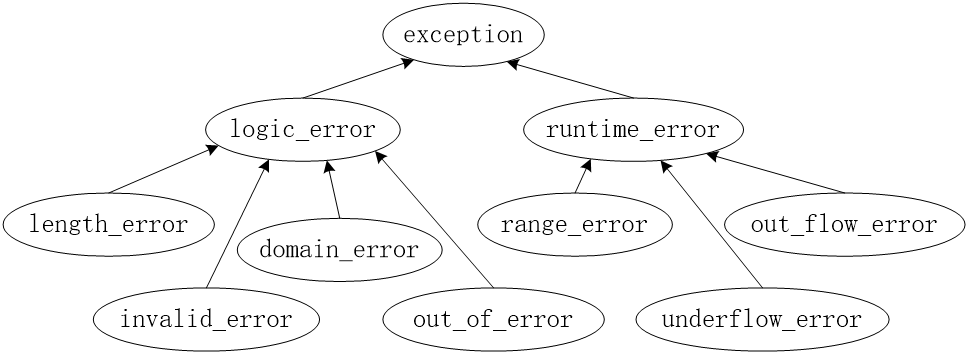
\includegraphics[scale=0.4]{Fig12-1.png}
    \end{figure}
    \begin{block}
        {基类exception}
        基类exception只定义了默认的构造函数、复制构造函数、赋值运算符、虚析构函数和一个名为\textbf{what}的虚成员。
    \end{block}
\end{frame}

\begin{frame}[fragile]{12.2~异常处理\small{——标准库异常类}}
    \textbf{what函数}返回一个const char*,指向一个以null结尾的字符数组,用于提示异常类型。我们可以继承exception类并\alert{重写what}:\\
    \begin{columns}[T]
        \column{0.65\textwidth}
        \begin{blueblock}
            {自定义版本的what成员}
            \begin{lstlisting}[moreemph={T}]
struct MyException :public exception {
    const char* what() const noexcept { return "Ooops!"; }
};
        \end{lstlisting}
        \end{blueblock}
        \column{0.3\textwidth}
        \begin{block}
            {noexcept}
            C++11标准引入的新关键字,用来指明某个函数\alert{不会抛出异常}
        \end{block}
        \only<1>{\begin{yellowblock}
                {说明}
                noexcept应置于:\\
                $\bullet$ 形参列表后面\\
                $\bullet$ 如修饰成员函数,在const限定符之后,final、override或纯虚函数=0之前\\
                $\bullet$ 声明和定义处都要有\\
            \end{yellowblock}}
        \only<2->{
            \begin{redblock}
                {提示}
                noexcept说明可以优化代码的执行效率。
            \end{redblock}
        }
    \end{columns}
\end{frame}

\begin{frame}[fragile]{12.2~异常处理\small{——标准库异常类}}
    下面的代码将抛出一个MyException异常对象,该对象可以被异常声明为\alert{基类exception}类型的catch子句捕获:\\
    \begin{columns}[T]
        \column{0.65\textwidth}
        \begin{blueblock}
            {使用MyException对象}
            \begin{lstlisting}[moreemph={T}]
try {
    throw MyException();
}
catch (exception &ex) {
    cerr << ex.what() << endl;
    }
\end{lstlisting}
        \end{blueblock}
        \column{0.3\textwidth}
    \end{columns}
\end{frame}

\section{多重继承与虚继承}
\subsection{多重继承}
\begin{frame}[fragile]{12.3~多重继承与虚继承\small{——多重继承}}
    \begin{block}
        {{12.1~命名空间\small{——使用命名空间}}}
        为一个派生类指定多个基类的继承结构称为{12.1~命名空间\small{——使用命名空间}}
    \end{block}
    \begin{columns}[T]
        \column{0.65\textwidth}
        \begin{blueblock}
            {{12.1~命名空间\small{——使用命名空间}}}
            \begin{lstlisting}[moreemph={T}]
class Mammal {
public:
    virtual void feedMilk() {} //母乳喂养
};
class WingedAnimal {
public:
    virtual void flap() {} //振翅飞翔
};
class Bat: public Mammal, public WingedAnimal { };
        \end{lstlisting}
        \end{blueblock}
        \column{0.3\textwidth}
        \begin{yellowblock}
            {说明}
            $\bullet$ Bat类的派生列表中有两个以逗号分隔的基类\\
            $\bullet$ Bat类对象将具有Mammal和WingedAnimal两种动物的行为\\
        \end{yellowblock}
    \end{columns}
\end{frame}

\begin{frame}[fragile]{12.3~多重继承与虚继承\small{——多重继承}}
    \begin{block}
        {多重继承}
        为一个派生类指定多个基类的继承结构称为多重继承
    \end{block}
    \begin{columns}[T]
        \column{0.65\textwidth}
        \begin{blueblock}
            {多重继承}
            \begin{lstlisting}[moreemph={T}]
Bat b;
b.feedMilk(); //母乳喂养
b.flap(); //振翅飞翔
        \end{lstlisting}
        \end{blueblock}
        \column{0.3\textwidth}
        \begin{yellowblock}
            {说明}
            $\bullet$ Bat类的派生列表中有两个以逗号分隔的基类\\
            $\bullet$ Bat类对象将具有Mammal和WingedAnimal两种动物的行为\\
        \end{yellowblock}
    \end{columns}
\end{frame}

\begin{frame}[fragile]{12.3~多重继承与虚继承\small{——多重继承}}
    \begin{columns}[T]
        \column{0.65\textwidth}
        \begin{blueblock}
            {多重继承}
            \begin{lstlisting}[moreemph={T}]
class Bat: public Mammal, public WingedAnimal { };
        \end{lstlisting}
        \end{blueblock}
        \begin{blueblock}
            {调用基类构造函数}
            \begin{lstlisting}[moreemph={T}]
//隐式调用Mammal和WingedAnimal的默认构造函数
Bat::Bat() {}
//显式调用基类的默认构造函数
Bat::Bat() :Mammal(), WingedAnimal() {}
        \end{lstlisting}
        \end{blueblock}
        \column{0.3\textwidth}
        \begin{yellowblock}
            {说明}
            $\bullet$ 多重继承的派生类对象的构造函数只能初始化其\alert{直接基类}成员\\
            $\bullet$ 构造的顺序与\alert{派生列表}中基类出现的先后顺序一致\\
            $\bullet$ 成员析构的顺序与构造的顺序相反\\
            $\bullet$ 调用基类的构造函数有\alert{隐式和显式}两种方式\\
        \end{yellowblock}
    \end{columns}
\end{frame}

\subsection{虚继承}
\begin{frame}[fragile]{12.3~多重继承与虚继承\small{——多重继承}}
    我们将Mammal和WingedAnimal进一步抽象,设计一个公共基类Animal:
    \begin{columns}[T]
        \column{0.65\textwidth}
        \begin{blueblock}
            {加入公共基类Animal}
            \begin{lstlisting}[moreemph={T}]
class Animal {
protected:
    int m_age;
public:
    Animal(int n = 0) :m_age(n) {}
    virtual void eat() {}
};
class WingedAnimal: public Animal{
public:
    virtual void feedMilk() {}
};
class Mammal: public Animal{
public:
    virtual void flap() {}
};
class Bat: public Mammal, public WingedAnimal { };
        \end{lstlisting}
        \end{blueblock}
        \column{0.3\textwidth}
        \begin{figure}
            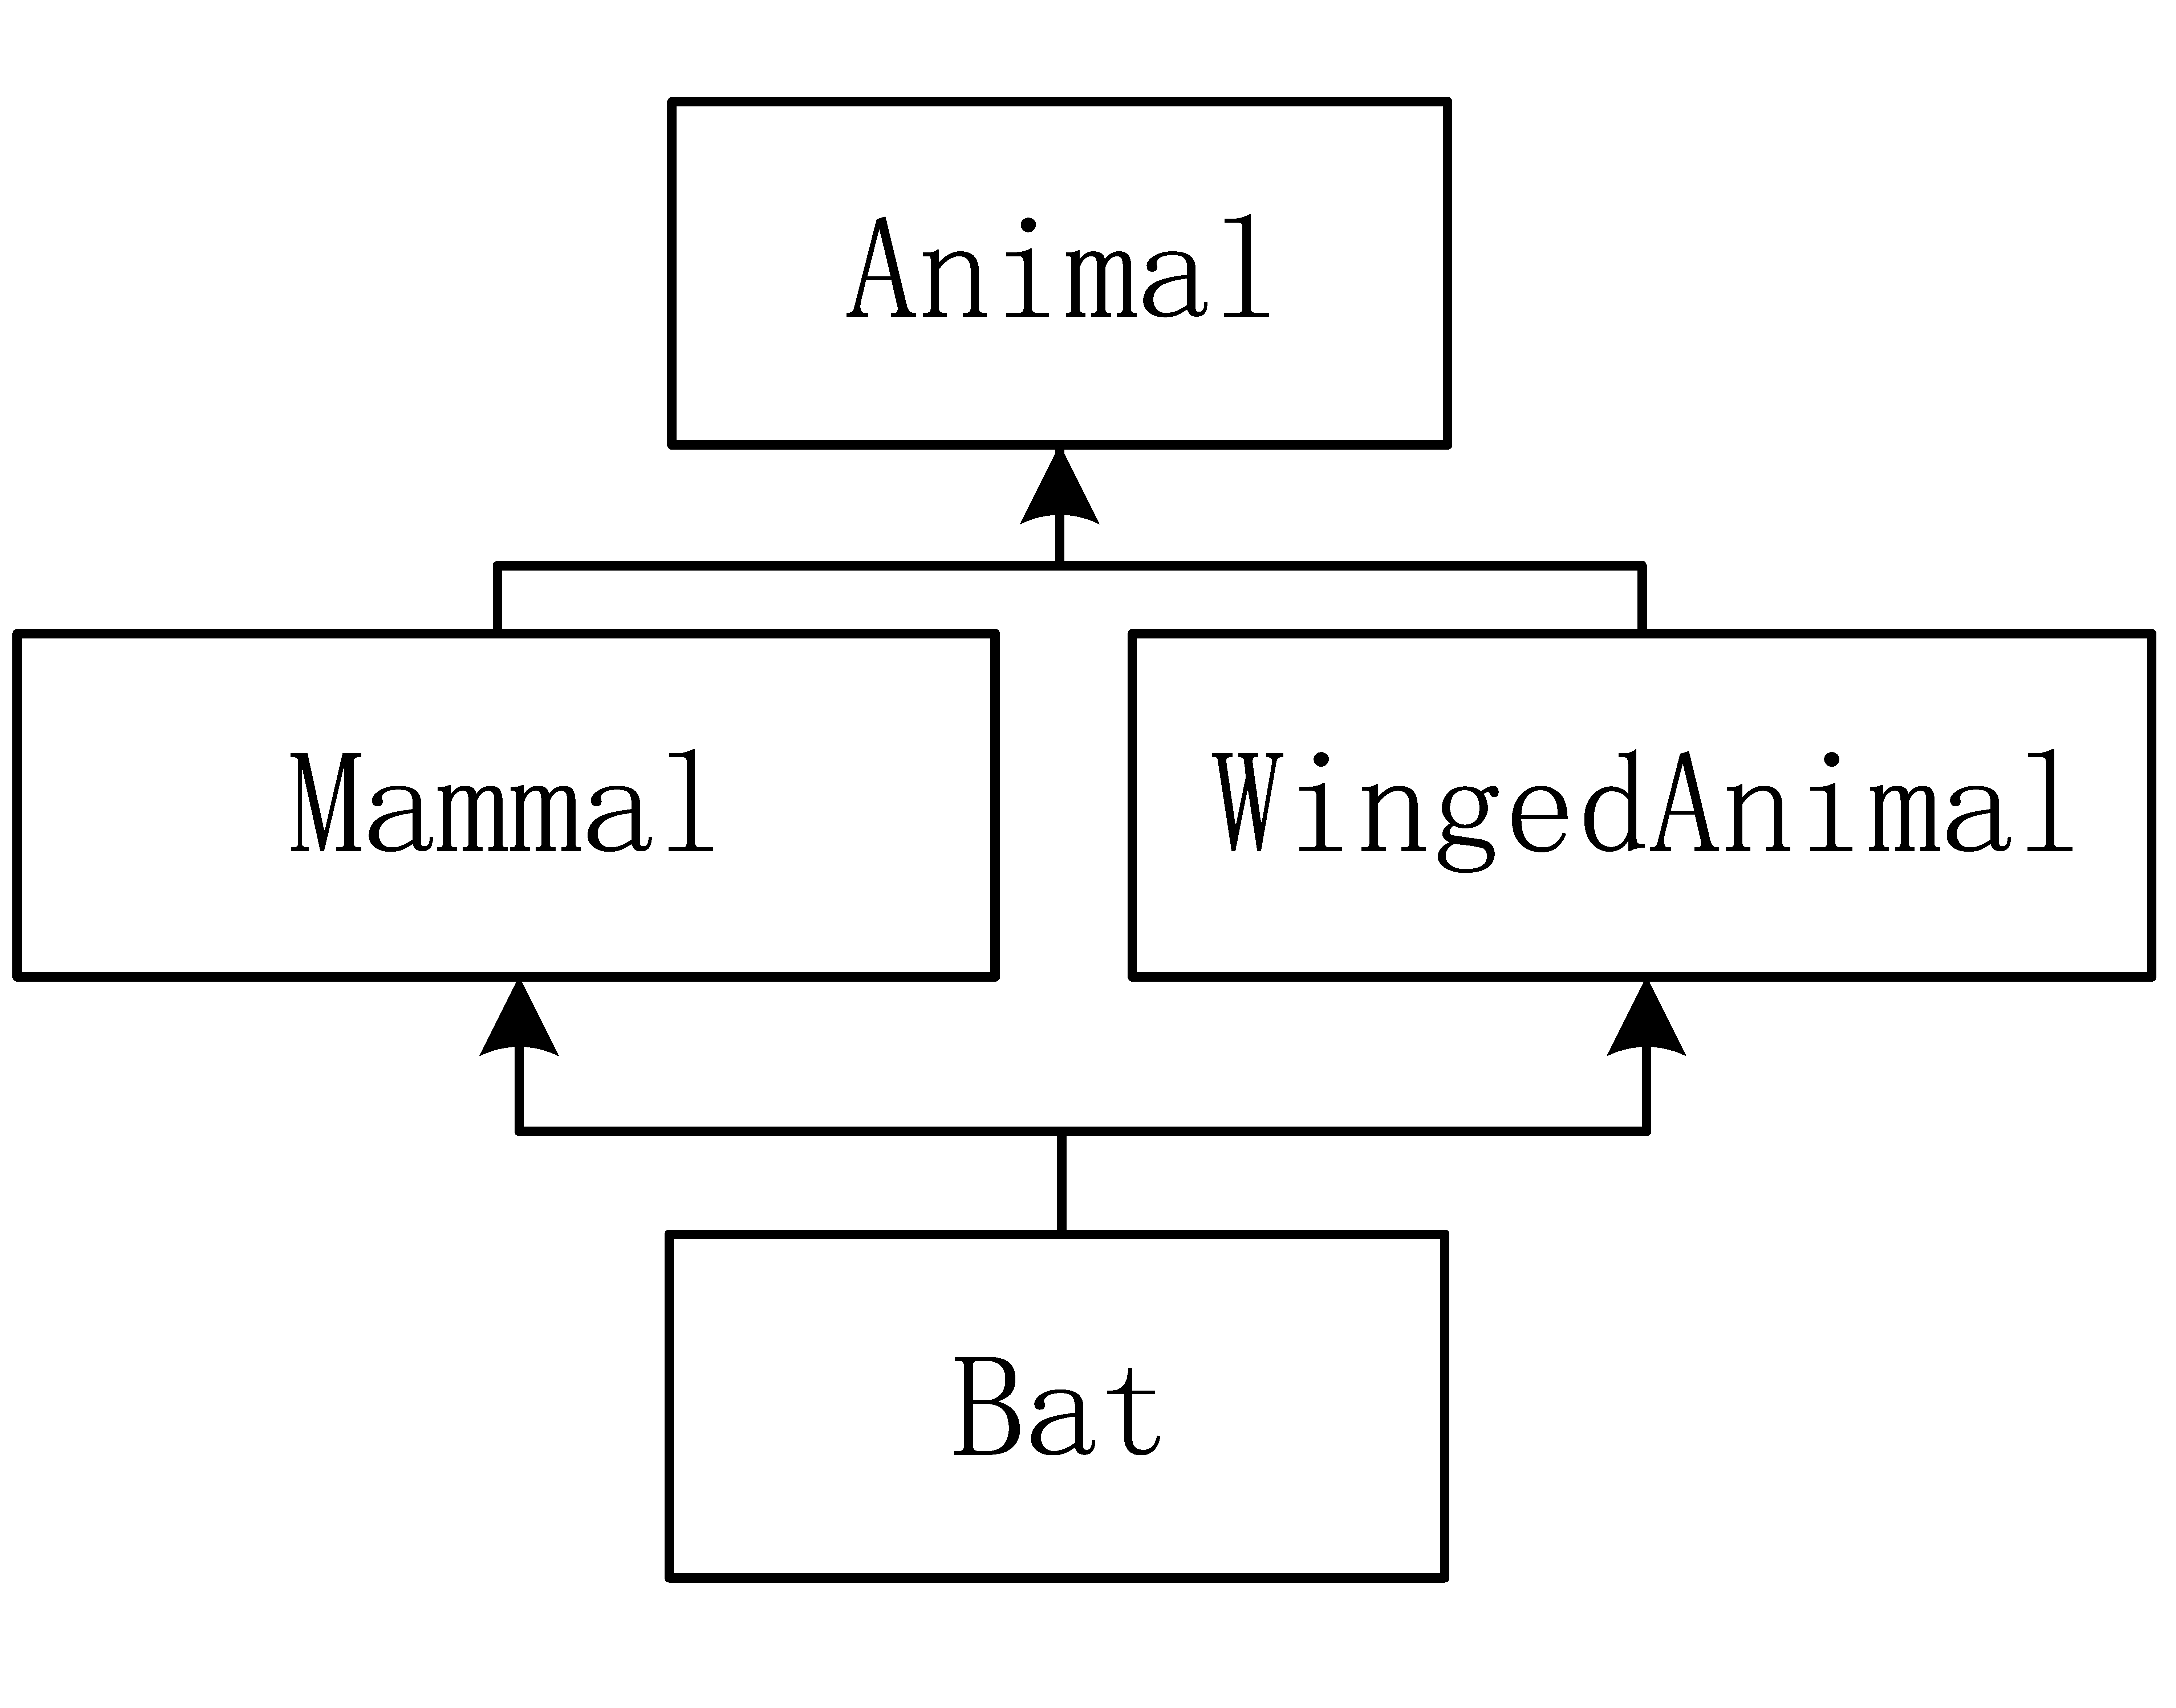
\includegraphics[scale=0.6]{Fig12-2.png}
        \end{figure}
        \begin{redblock}
            {死亡钻石}
            菱形继承关系造成的二义性问题
        \end{redblock}
    \end{columns}
\end{frame}

\begin{frame}[fragile]{12.3~多重继承与虚继承\small{——多重继承}}
    当存在如下调用的时候,会产生二义性问题:
    \begin{columns}[T]
        \column{0.65\textwidth}
        \begin{blueblock}
            {加入公共基类Animal}
            \begin{lstlisting}[moreemph={T}]
Bat b;
b.eat(); //错误:二义性访问
Animal a = b; //错误:类型无法转换
        \end{lstlisting}
        \end{blueblock}
        \column{0.35\textwidth}
    \end{columns}
\end{frame}

\begin{frame}[fragile]{12.3~多重继承与虚继承\small{——多重继承}}
    C++通过\textbf{虚继承(virtual inheritance)}的机制来解决上述问题:
    \begin{columns}[T]
        \column{0.65\textwidth}
        \begin{blueblock}
            {加入公共基类Animal}
            \begin{lstlisting}[moreemph={T}]
class WingedAnimal: virtual public Animal {/*...*/};
class Mammal : virtual public Animal {/*...*/};
        \end{lstlisting}
        \end{blueblock}
        \column{0.3\textwidth}
        \begin{yellowblock}
            {说明}
            $\bullet$ 通过在派生列表中添加关键字\alert{virtual}来指定虚基类\\
            $\bullet$ 不论该虚基类在继承体系中出现多少次,在派生类中只包含\alert{唯一一份}共享的虚基类成员\\
        \end{yellowblock}
    \end{columns}
\end{frame}

\begin{frame}[fragile]{12.3~多重继承与虚继承\small{——多重继承}}
    虚继承的基类由\alert{最底层的派生类进行初始化}:
    \begin{columns}[T]
        \column{0.65\textwidth}
        \begin{blueblock}
            {虚继承对象的构造}
            \begin{lstlisting}[moreemph={T}]
class Bat : public Mammal, public WingedAnimal {
public:
    Bat() :Animal(1), Mammal(), WingedAnimal(){}
};
        \end{lstlisting}
        \end{blueblock}
        \column{0.3\textwidth}
        \begin{yellowblock}
            {说明}
            此处初始化顺序如下:\\
            $\bullet$ Bat类的构造函数提供的初始化列表初始化Animal成员\\
            $\bullet$ 构造Mammal成员\\
            $\bullet$ 构造WingedAnimal成员\\
        \end{yellowblock}
    \end{columns}
\end{frame}

\section{嵌套类}
\begin{frame}[fragile]{12.4~嵌套类}
    \begin{block}
        {嵌套类}
        在一个类的内部定义的类
    \end{block}
    \begin{yellowblock}
        {说明}
        $\bullet$ 嵌套类是\alert{独立}的类,与外层类在语法上没有关联\\
        $\bullet$ 嵌套类和外层类的访问控制遵循\alert{普通类}之间的访问控制原则\\
    \end{yellowblock}
\end{frame}

\subsection{二维数组类}
\begin{frame}[fragile]{12.4~嵌套类\small{——二维数组类}}
    \begin{greenblock}
        {任务}
        实现一个二维数组类,该类可以像普通二维数组那样支持两个下标操作:
        \begin{lstlisting}[moreemph={T}]
int arr[2][2];
arr[0][0] = 1;
\end{lstlisting}
    \end{greenblock}

    \begin{greenblock}
        {存在的难点}
        C++仅支持一维下标操作符的重载:
        \begin{lstlisting}[moreemph={T}]
class Array2D{
    /*...*/
    int operator [][](/*...*/); //错误:C++没有运算符[][]
};
\end{lstlisting}
    \end{greenblock}

    \onslide<2>{\begin{yellowblock}
            {分析}
            \texttt{arr[0][0]}等价于\texttt{(arr[0])[0]}
        \end{yellowblock}}
\end{frame}

\begin{frame}[fragile]{12.4~嵌套类\small{——二维数组类}}
    \begin{blueblock}
        {代码清单12.1~二维数组类}
        \begin{lstlisting}[moreemph={T}]
template<typename T>
class Array2D {
private:
    class Array1D {
        ... //下页内容
    };
    size_t m_size; //第一维长度
    Array1D *m_arr; //元素类型为Array1D
    public:
    Array2D(size_t s1, size_t s2) :m_size(s1), m_arr(new Array1D[s1]) {
        for (int i = 0; i<m_size; i++) {
            m_arr[i].m_size = s2;
            m_arr[i].m_arr = new T[s2];
        }
    }
    ~Array2D() { delete[] m_arr; }
    Array1D & operator[](int idx) { return m_arr[idx]; }
    size_t size() { return m_size; }
};
        \end{lstlisting}
    \end{blueblock}
\end{frame}

\begin{frame}[fragile]{12.4~嵌套类\small{——二维数组类}}
    \begin{columns}[T]
        \column{0.65\textwidth}
        \begin{blueblock}
            {代码清单12.1~二维数组类}
            \begin{lstlisting}[moreemph={T}]
...//上页内容
class Array1D {
    friend class Array2D; //声明为友元类
public:
    ~Array1D() { delete[] m_arr; }
    T & operator[](int idx) { return m_arr[idx]; }
private:
    size_t m_size = 0; //第二维长度
    T *m_arr = nullptr;
};
...//上页内容
\end{lstlisting}
        \end{blueblock}
        \begin{blueblock}
            {使用二维数组}
            \begin{lstlisting}[moreemph={T}]
Array2D<int> arr(2, 2);
arr[0][0] = 1;
\end{lstlisting}
        \end{blueblock}
        \column{0.3\textwidth}
        \begin{yellowblock}
            {说明}
            $\bullet$ 使用嵌套类将Array1D的底层实现隐藏
        \end{yellowblock}
    \end{columns}
\end{frame}

\subsection{通用计算器}
\begin{frame}[fragile]{12.4~嵌套类\small{——二维数组类}}
    9.3.5节中我们实现的计算器程序有以下的代码:
    \begin{columns}[T]
        \column{0.65\textwidth}
        \begin{blueblock}
            {计算器}
            \begin{lstlisting}[moreemph={T}]
/*...*/
unique_ptr<Operator> oo;
if (o == ’+’)
    oo = make_unique<Plus>();
else if (o == ’-’)
    oo = make_unique<Minus>();
/*...*/
\end{lstlisting}
        \end{blueblock}
        \column{0.3\textwidth}
        \begin{greenblock}
            {思考}
            如果我们想要为计算器添加新的运算符,我们要怎么做?
        \end{greenblock}
    \end{columns}
\end{frame}


\begin{frame}[fragile]{12.4~嵌套类\small{——二维数组类}}
    为了有利程序扩展,我们希望\alert{根据运算符的名字来自动创建相应运算符类对象}。
    首先我们需要实现一个\textbf{类注册机制},我们将用如下数据结构来实现:
    \begin{columns}[T]
        \column{0.65\textwidth}
        \begin{blueblock}
            {类注册机制核心数据结构}
            \begin{lstlisting}[moreemph={T}]
map<char, function<unique_ptr<Operator>()>> ms_operator;
\end{lstlisting}
        \end{blueblock}
        \column{0.3\textwidth}
        \begin{block}
            {类注册机制}
            保存\alert{类名(字符串)}和\alert{类实例}获取方法的映射关系,使程序能够根据名称得到类的实例。
        \end{block}
    \end{columns}
    \begin{yellowblock}
        {说明}
        $\bullet$ map对象的关键字为char类型,用于根据字符调用对应的function对象\\
        $\bullet$ function对象将返回一个指向Operator对象的unique\_ptr,用于生成对应运算符对象\\
    \end{yellowblock}
\end{frame}

\begin{frame}[fragile]{12.4~嵌套类\small{——二维数组类}}
    下面代码将自动注册Plus类:
    \begin{columns}[T]
        \column{0.65\textwidth}
        \begin{blueblock}
            {类注册机制核心数据结构}
            \begin{lstlisting}[moreemph={T}]
ms_operator.emplace(’+’,[]() { return make_unique<Plus>(); });
\end{lstlisting}
        \end{blueblock}
        \column{0.3\textwidth}
        \begin{yellowblock}
            {说明}
            $\bullet$ emplace函数用于向map插入一组char到Operator对象生成器的映射\\
            $\bullet$ lambda表达式用于初始化function对象
        \end{yellowblock}
    \end{columns}
    \vspace{0.5cm}
\end{frame}

\begin{frame}[fragile]{12.4~嵌套类\small{——二维数组类}}
之后即可根据用算符名字自动创建该运算符类对象:
\begin{blueblock}
    {类注册机制核心数据结构}
    \begin{lstlisting}[moreemph={T}]
ms_operator.emplace(’+’,[]() { return make_unique<Plus>(); });
\end{lstlisting}
\end{blueblock}
\begin{blueblock}
    {根据名字自动创建运算符}
    \begin{lstlisting}[moreemph={T}]
unique_ptr<Operator> oo = ms_operator[’+’]();
\end{lstlisting}
\end{blueblock}
\begin{yellowblock}
    {说明}
    $\bullet$ 下标运算符调用function对象\\
    $\bullet$ function对象通过lambda表达式调用make\_unique\\
    $\bullet$ make\_unique将返回对应下标运算符接收的字符所对应的Operator的unique\_ptr\\
\end{yellowblock}
\end{frame}

\begin{frame}[fragile]{12.4~嵌套类\small{——二维数组类}}
    为了方便用户注册,我们实现一个\textbf{对象工厂(object factory)}:
    \begin{columns}[T]
        \column{0.65\textwidth}
        \begin{blueblock}
            {代码清单12.2 Operator类对象工厂1}
            \begin{lstlisting}[moreemph={T}]
class Factory{
public:
template<typename T>
struct RegisterClass {
    RegisterClass(char opr) {
        Factory::ms_operator.emplace(opr,
          []{return make_unique<T>();});
    } //在ms_operator作用域范围内,可以直接访问
};
static unique_ptr<Operator> create(char opr) {
    auto it = ms_operator.find(opr);
    if (it != ms_operator.end())
        return it->second(); //调用关联的lambda表达式
}
private://静态成员
    static map<char,
      function<unique_ptr<Operator>()>> ms_operator;
};
\end{lstlisting}
        \end{blueblock}
        \column{0.3\textwidth}
        \begin{yellowblock}
            {说明}
            $\bullet$ 工厂通过嵌套类RegisterClass的构造函数实现对其静态成员ms\_operator的类型注册功能\\
            $\bullet$ it->second()调用与opr相关的lambda表达式,返回对应的对象。\\
        \end{yellowblock}
    \end{columns}
    \vspace{0.5cm}
\end{frame}

\begin{frame}[fragile]{12.4~嵌套类\small{——二维数组类}}
    下面是用于注册的宏和静态成员的初始化:
    \begin{columns}[T]
        \column{0.65\textwidth}
        \begin{blueblock}
            {代码清单12.2 Operator类对象工厂2}
            \begin{lstlisting}[moreemph={T}]
#define REGISTRAR(T, Key) Factory::RegisterClass<T> reg_##T(Key);
map<char, function<unique_ptr<Operator>()>> Factory::ms_operator;
\end{lstlisting}
        \end{blueblock}
        \begin{blueblock}
            {示例:注册Plus类}
            \begin{lstlisting}[moreemph={T}]
REGISTRAR(Plus, ’+’);
\end{lstlisting}
            等价于:
            \begin{lstlisting}[moreemph={T}]
Factory::RegisterClass<Plus> reg_Plus(’+’);
\end{lstlisting}
        \end{blueblock}

        \column{0.3\textwidth}
        \begin{yellowblock}
            {说明}
            $\bullet$ 通过宏REGISTRAER创建嵌套类RegisterClass的全局对象同时完成注册\\
            $\bullet$ \texttt{\#\#}用来连接两个语言符号,产生一个对象名\\
            $\bullet$ lambda表达式用于初始化function对象\\
        \end{yellowblock}
    \end{columns}
\end{frame}

\begin{frame}[fragile]{12.4~嵌套类\small{——二维数组类}}
    其他运算符类注册方式类似:
    \begin{columns}[T]
        \column{0.65\textwidth}
        \begin{blueblock}
            {代码清单12.2 Operator类对象工厂2}
            \begin{lstlisting}[moreemph={T}]
REGISTRAR(Minus, ’-’);
REGISTRAR(Multiply, ’*’);
REGISTRAR(Divide, ’/’);
REGISTRAR(Equal, ’=’);
\end{lstlisting}
        \end{blueblock}
        \column{0.3\textwidth}
        \begin{yellowblock}
            {说明}
            $\bullet$ 通过宏REGISTRAER创建嵌套类RegisterClass的全局对象同时完成注册\\
            $\bullet$ \texttt{\#\#}用来连接两个语言符号,产生一个对象名\\
            $\bullet$ lambda表达式用于初始化function对象\\
        \end{yellowblock}
    \end{columns}
\end{frame}

\begin{frame}[fragile]{12.4~嵌套类\small{——二维数组类}}
    \begin{columns}[T]
        \column{0.65\textwidth}
        \begin{blueblock}
            {修改后Calculator类的doIt函数}
            \begin{lstlisting}[moreemph={T}]
double Calculator::doIt(const string & exp) {
    for (auto it = exp.begin(); it != exp.end();) {
        if (isNum(it))
            m_num.push(readNum(it));
        else {
            auto oo=Factory::create(*it++);
            while (oo->precedence() <= m_opr.top()->precedence()) {
                if (m_opr.top()->symbol() == ’#’)
                    break;
                calculate();
            }
            if (oo->symbol() != ’=’)
                m_opr.push(std::move(oo));
        }
    }
    double result = m_num.top();
    m_num.pop();
    return result;
}
\end{lstlisting}
        \end{blueblock}
        \column{0.3\textwidth}
        \begin{yellowblock}
            {说明}
            第6行代码调用Factory::create函数,用来构造相应类型的对象\\
        \end{yellowblock}
        \begin{greenblock}
            {问题}
            如果形参未注册,调用create将会返回什么?
        \end{greenblock}
        \pause
        \begin{greenblock}
            {思考}
            体会修改后代码和原始代码的区别以及改进之处
        \end{greenblock}
    \end{columns}
\end{frame}

\section{运行时类型识别}
\begin{frame}[fragile]{12.5~运行时类型识别}
    \begin{block}
        {运行时类型识别}
        运行时类型识别(run-time type identification, RTTI)指的是通过\alert{基类的指针或引用}来检查其指向的\alert{派生类型}。
    \end{block}
    RTTI提供如下两个运算符:
    \begin{itemize}
        \item \texttt{typeid}
        \item \texttt{dynamic\_cast}
    \end{itemize}
    \vspace{0.5cm}
    这两个运算符作用于基类的指针或引用,如果该类型:
    \begin{itemize}
        \item 含有虚函数,则返回\alert{基类指针或引用的动态类型}
        \item 不含有虚函数,则返回\alert{该类型的静态类型}
    \end{itemize}
\end{frame}



\subsection{dynamic\_cast运算符}
\begin{frame}[fragile]{12.5~运行时类型识别\small{——dynamic\_cast运算符}}
    \textbf{dynamic\_cast运算符}用于\alert{基类和派生类}之间的安全转换,其使用方式有:
    \begin{columns}[T]
        \column{0.65\textwidth}
        \begin{blueblock}
            {dynamic\_cast用法}
            \begin{lstlisting}[moreemph={T}]
dynamic_cast<type*>(expr)
dynamic_cast<type&>(expr)
dynamic_cast<type&&>(expr)
\end{lstlisting}
        \end{blueblock}
        \column{0.3\textwidth}
        \begin{yellowblock}
            {说明}
            三种使用方式中,expr依次必须为:\\
            $\bullet$ 有效的指针\\
            $\bullet$ 左值\\
            $\bullet$ 右值\\
        \end{yellowblock}
    \end{columns}
    \begin{redblock}
        {注意}
        成功转换的前提:\\
        expr的类型必须是type的基类、派生类或type本身\\
        否则:\\
        $\bullet$ 指针类型返回空指针\\
        $\bullet$ 引用类型抛出std::bad\_cast异常\\
    \end{redblock}
\end{frame}

\begin{frame}[fragile]{12.5~运行时类型识别\small{——dynamic\_cast运算符}}
    dynamic\_cast运算符用于\alert{基类和派生类}之间的安全转换,其使用方式有:
    \begin{columns}[T]
        \column{0.65\textwidth}
        \begin{blueblock}
            {定义基类及其派生类}
            \begin{lstlisting}[moreemph={T}]
struct Base{
    virtual ~Base() {}
};
struct Derived:Base{
    void name() {}
};
\end{lstlisting}
        \end{blueblock}
        \begin{blueblock}
            {指针类型的dynamic\_cast}
            \begin{lstlisting}[moreemph={T}]
Base *b1 = new Base, *b2 = new Derived;
if (Derived *d = dynamic_cast<Derived*>(b1))
    d->name(); //转换失败,d为nullptr,不会执行此调用
if (Derived *d = dynamic_cast<Derived*>(b2))
    d->name(); //转换成功,执行此调用
\end{lstlisting}
        \end{blueblock}
        \column{0.3\textwidth}
        \begin{yellowblock}
            {说明}
            下方代码:\\
            $\bullet$ 第一个转换b1与基类对象绑定,转换失败\\
            $\bullet$ 第二个转换b2与派生类对象绑定,转换成功,执行name调用\\
        \end{yellowblock}
        \begin{redblock}
            {建议}
            把dynamic\_cast操作放到条件定义里,避免出现\alert{使用未绑定指针}的不安全操作
        \end{redblock}
    \end{columns}
\end{frame}

\begin{frame}[fragile]{12.5~运行时类型识别\small{——dynamic\_cast运算符}}
    dynamic\_cast运算符用于\alert{基类和派生类}之间的安全转换,其使用方式有:
    \begin{columns}[T]
        \column{0.65\textwidth}
        \begin{blueblock}
            {引用类型的dynamic\_cast}
            \begin{lstlisting}[moreemph={T}]
try { //转换失败,抛出std::bad_cast异常
    Derived &d = dynamic_cast<Derived&>(*b1);
}catch(std::bad_cast){
    cout << "downcast failed" << endl;
}
\end{lstlisting}
        \end{blueblock}
        \column{0.3\textwidth}
        \begin{yellowblock}
            {说明}
            引用类型的dynamic\_cast转换失败时将抛出std::bad\_cast异常\\
        \end{yellowblock}
    \end{columns}
\end{frame}

\subsection{typeid运算符}
\begin{frame}[fragile]{12.5~运行时类型识别\small{——typeid运算符}}
    \textbf{关键字\texttt{typeid}}用来查询一个类型的信息
    \begin{blueblock}
        {typeid使用格式}
        \begin{lstlisting}[moreemph={T}]
typeid(type)
typeid(expr)
\end{lstlisting}
    \end{blueblock}
    \begin{yellowblock}
        {说明}
        \begin{itemize}
            \item 如果表达式类型是\alert{类类型且包含虚成员函数},那么需要在\alert{运行时}计算并返回表达式的\alert{动态类型};
            \item 否则,typeid运算将返回表达式的\alert{静态类型},在\alert{编译时}获得。
        \end{itemize}
    \end{yellowblock}
\end{frame}

\begin{frame}[fragile]{12.5~运行时类型识别\small{——typeid运算符}}
    typeid操作符的返回结果是名为type\_info 的标准库类型对象的引用。其支持的操作如下:
        \begin{blueblock}
            {typeid使用格式}
            \begin{lstlisting}[moreemph={T}]
t1 == t2      如果两个type_info对象t1和t2类型相同,则返回真;否则返回假
t1 != t2      如果两个type_info对象t1和t2类型不同,则返回真;否则返回假
t.name()      返回类型的C风格字符串,类型名字用系统相关的方法产生
t1.before(t2) 返回一个bool值,表示t1类型是否出现在t2类型之前
\end{lstlisting}
        \end{blueblock}
        \begin{redblock}
            {注意}
            name成员返回的类型名与程序中使用的类型名并不一定一致,具体由编译器的实现决定\\
        \end{redblock}
\end{frame}

\begin{frame}[fragile]{12.5~运行时类型识别\small{——typeid运算符}}
    typeid常用于比较两个表达式的类型是否相同,或一个表达式的类型是否与指定类型一致:
        \begin{blueblock}
            {typeid比较}
            \begin{lstlisting}[moreemph={T}]
Derived *d = new Derived;
Base *b = d;
if (typeid(*d) == typeid(*b)) { /*检查d和p是否指向同一类型对象*/}
if (typeid(*b) == typeid(Derived)) {/*检查b是否指向Derived类型对象*/}
\end{lstlisting}
        \end{blueblock}
        \begin{redblock}
            {注意}
            此处typeid作用于*b而非b。\\
        \end{redblock}
\end{frame}

\section{union类型}
\begin{frame}[fragile]{12.6~union类型}
    \begin{block}
        {union类型}
        一种特殊的复合数据类型,可以实现一个对象用作多种数据类型的作用
    \end{block}
    \begin{yellowblock}
        {说明}
        $\bullet$ 可以包含多个\alert{共享同一段内存空间}的数据成员\\
        $\bullet$ 占用的空间大小取决于\alert{内存占用最大}的数据成员类型\\
        $\bullet$ 使用时\alert{只有一个数据成员}处于激活状态\\
    \end{yellowblock}
\end{frame}

\subsection{定义union类型}
\begin{frame}[fragile]{12.6~union类型\small{——定义union类型}}
    union类型定义方法
    \begin{columns}[T]
        \column{0.65\textwidth}
        \begin{blueblock}
            {union类型定义}
            \begin{lstlisting}[moreemph={T}]
union ID {
    char char_type;
    int int_type;
    long long llong_type;
};
\end{lstlisting}
        \end{blueblock}
        \column{0.3\textwidth}
        \begin{yellowblock}
            {说明}
            $\bullet$ 定义了名为ID的union类型\\
            $\bullet$ ID类对象可用于存储char、int、long类型数据\\
            $\bullet$ ID类型对象占用内存长度和long类型长度相同\\
        \end{yellowblock}
    \end{columns}
\end{frame}

\subsection{使用union类型}
\begin{frame}[fragile]{12.6~union类型\small{——使用union类型}}
    union类型定义方法:
    \begin{columns}[T]
        \column{0.65\textwidth}
        \begin{blueblock}
            {union类型定义}
            \begin{lstlisting}[moreemph={T}]
ID wang = {’a’}; //构造一个ID类对象并为第一个成员赋值
cout << wang.char_type << endl; //输出a
wang.int_type = 1001; //激活使用第二个成员
cout << wang.int_type << endl; //输出1001
wang.llong_type = 20171001001; //激活使用第三个成员
cout << wang.llong_type << endl; //输出20171001001
\end{lstlisting}
        \end{blueblock}
        \column{0.3\textwidth}
        \begin{yellowblock}
            {说明}
            $\bullet$ 使用花括号可对其\alert{第一个}数据成员赋值\\
            $\bullet$ 赋值后其他成员将处于\alert{未定义}状态\\
            $\bullet$ ID类型对象占用内存长度和long类型长度相同\\
        \end{yellowblock}
    \end{columns}
\end{frame}

\begin{frame}[fragile]{12.6~union类型\small{——使用union类型}}
    \begin{redblock}
            {注意}
            class的大多特征适用于union:\\
            $\bullet$ 其数据成员可用private、public和protected修饰,默认为public\\
            $\bullet$ 可以定义成员函数\\
            但另一些特征union不具备:\\
            $\bullet$ 不能包含引用类型的数据成员\\
            $\bullet$ union类不具备继承特性\\
        \end{redblock}
    \begin{redblock}
            {注意}
            另外:\\
            $\bullet$ 如成员为类类型,状态变化时将调用其构造/析构函数\\
            $\bullet$ 使用时必须清楚使用的是哪一个成员,错误使用会导致崩溃\\
        \end{redblock}
\end{frame}

\section{标准库特殊工具}
\subsection{tuple类型}
\begin{frame}[fragile]{12.7~标准库特殊工具\small{——tuple类型}}
    \begin{block}
        {tuple}
        tuple(元组)是固定大小的异类值集合,它是泛化的pair
    \end{block}
    \begin{columns}[T]
        \column{0.65\textwidth}
        \begin{blueblock}
            {定义tuple对象}
            \begin{lstlisting}[moreemph={T}]
tuple<string, double, int,list<string>> book(
  "title1",58.99,2017,{"Mandy","Lisha","Rosieta"});
\end{lstlisting}
        \end{blueblock}
        \column{0.3\textwidth}
        \begin{yellowblock}
            {说明}
            tuple对象必须\alert{直接初始化}\\
        \end{yellowblock}
    \end{columns}
    \begin{columns}[T]
        \column{0.65\textwidth}
        \begin{blueblock}
            {make\_tuple函数}
            \begin{lstlisting}[moreemph={T}]
auto book2 = make_tuple(string("title2"), 68.99, 2017, list<string>{"Mandy","Lisha","Rosieta"});
\end{lstlisting}
        \end{blueblock}
        \column{0.3\textwidth}
        \begin{yellowblock}
            {说明}
            make\_tuple使我们可以利用\alert{auto推导类型}而不必显式指定\\
        \end{yellowblock}
    \end{columns}
\end{frame}

\begin{frame}[fragile]{12.7~标准库特殊工具\small{——tuple类型}}
        \begin{blueblock}
            {访问tuple成员}
            \begin{lstlisting}[moreemph={T}]
auto item1= get<0>(book); //访问第一个元素
get<1>(book) = 48.99; //对第二个元素赋值
for (auto &i : get<3>(book)) //使用范围for访问第四个成员的所有元素
    cout << i << " ";
\end{lstlisting}
        \end{blueblock}
        \begin{yellowblock}
            {说明}
            $\bullet$ 使用标准库函数模板get来获取tuple的成员\\
            $\bullet$ 使用get时需提供一个整型常量表达式实参,如\texttt{get<0>}表示第一个成员\\
        \end{yellowblock}
\end{frame}

\begin{frame}[fragile]{12.7~标准库特殊工具\small{——tuple类型}}
    \begin{columns}[T]
        \column{0.65\textwidth}
        \begin{blueblock}
            {比较tuple对象}
            \begin{lstlisting}[moreemph={T}]
if(book < book2) {/*...*/}
if(book == book2) {/*...*/}
\end{lstlisting}
        \end{blueblock}
        \column{0.3\textwidth}
        \begin{yellowblock}
            {说明}
            两个tuple可比较的条件:\\
            $\bullet$ 成员数量相等\\
            $\bullet$ 对应成员可以比较\\
            比较的规则为按\alert{字典顺序}比较tuple中的值\\
        \end{yellowblock}
    \end{columns}
\end{frame}

\begin{frame}[fragile]{12.7~标准库特殊工具\small{——tuple类型}}
    \begin{columns}[T]
        \column{0.65\textwidth}
        \begin{blueblock}
            {使用tie函数}
            \begin{lstlisting}[moreemph={T}]
string title;
double price;
int year;
list<string> author;
auto book3 = tie(title, price, year, author); //创建一个tuple对象
\end{lstlisting}
        \end{blueblock}
        \column{0.3\textwidth}
        \begin{yellowblock}
            {说明}
            标准库tie函数可以将多个对象的\alert{左值引用}组合为一个tuple对象
        \end{yellowblock}
    \end{columns}
    \begin{columns}[T]
        \column{0.65\textwidth}
        \begin{blueblock}
            {tuple对象的解包操作}
            \begin{lstlisting}[moreemph={T}]
tie(title, price, year, author) = book;
cout << title << " " << price << " "<< year;
\end{lstlisting}
            输出:
            \begin{lstlisting}[moreemph={T}]
title1 48.99 2017
    \end{lstlisting}
        \end{blueblock}
        \column{0.3\textwidth}
        \begin{yellowblock}
            {说明}
            $\bullet$ 第一条语句将book中的成员依次赋值给tie函数创建的tuple对象\\
            $\bullet$ 由于tie函数创建的tuple包含的是对象的引用,所以输出如上\\
        \end{yellowblock}
    \end{columns}
\end{frame}



\subsection{bitset类型}
\begin{frame}[fragile]{12.7~标准库特殊工具\small{——bitset类型}}
    \begin{block}
        {bitset}
        固定长度的二进制序列,可以方便地进行逻辑运算,及与字符串和整数相互转换。
    \end{block}
    \begin{columns}[T]
        \column{0.65\textwidth}
        \begin{blueblock}
            {定义bitset}
            \begin{lstlisting}[moreemph={T}]
bitset<12> b(1002); //b的二进制序列[0011 1110 1010]
bitset<12> b2("110010"); //二进制序列为[0000 0011 0010]
\end{lstlisting}
        \end{blueblock}
        \column{0.3\textwidth}
        \begin{yellowblock}
            {说明}
            $\bullet$ 模板参数为表示位长度的整型表达式\\
            $\bullet$ bitset可以由整型值初始化,整形将转换为unsigned long long再转化为位模式存储\\
            $\bullet$ bieset也可以由0和1组成的字符串常量初始化\\
        \end{yellowblock}
    \end{columns}
\end{frame}

\begin{frame}[fragile]{12.7~标准库特殊工具\small{——bitset类型}}
    \begin{block}
        {bitset}
        固定长度的二进制序列,可以方便地进行逻辑运算,及与字符串和整数相互转换。
    \end{block}
    \begin{columns}[T]
        \column{0.65\textwidth}
        \begin{blueblock}
            {高位舍弃}
            \begin{lstlisting}[moreemph={T}]
bitset<8> b1(1002); //舍弃高位,b1 的二进制序列[1110 1010]
\end{lstlisting}
        \end{blueblock}
        \column{0.3\textwidth}
        \begin{yellowblock}
            {说明}
            $\bullet$ unsigned long long位数如大于bitset长度,则高位会被舍弃\\
            $\bullet$ 否则多余高位设为0\\
        \end{yellowblock}
    \end{columns}
\end{frame}

\begin{frame}[fragile]{12.7~标准库特殊工具\small{——bitset类型}}
    bitset的一些成员函数如下所示:
    \begin{columns}[T]
        \column{0.45\textwidth}
        \begin{blueblock}
            {bitset成员函数——统计}
            \begin{lstlisting}[moreemph={T}]
bitset<8> b3("01010101");
b3.any(); //是否至少有一位为1
b3.none(); //是否所有位全为0
b3.all(); //是否所有位全为1
b3.count(); //值为1的位的数量
b3.size(); //位集合的长度
\end{lstlisting}
        \end{blueblock}
        \column{0.45\textwidth}
        \begin{blueblock}
            {bitset成员函数——位操作}
            \begin{lstlisting}[moreemph={T}]
b3.flip(); //所有位取反(0变1,1变0)
b3.reset(); //所有位设为0
b3.set(); //所有位设为1
b3.set(i); //第i位设为1
b3.reset(i); //第i位设为0
b3.flip(i); //第i位取反
b3.test(i); //第i 位是否为1
b3[i] = 0; //第i位设为0
\end{lstlisting}
        \end{blueblock}
    \end{columns}
\end{frame}

\begin{frame}[fragile]{12.7~标准库特殊工具\small{——bitset类型}}
    \begin{columns}[T]
        \column{0.65\textwidth}
        \begin{blueblock}
            {bitset转化为整型值}
            \begin{lstlisting}[moreemph={T}]
cout << b.to_ullong() << endl; //输出1002
\end{lstlisting}
        \end{blueblock}
        \column{0.3\textwidth}
        \begin{yellowblock}
            {说明}
            bitset的成员函数to\_ulong和to\_ullong可将位集合的二进制序列转化成整型值
        \end{yellowblock}
        \begin{redblock}
            {注意}
            待转换的位集合的长度不能大于long或long long的位数
        \end{redblock}
    \end{columns}
\end{frame}

\subsection{日期和时间}
\begin{frame}[fragile]{12.7~标准库特殊工具\small{——日期和时间}}
    C++提供\textbf{chrono库}对时间和日期进行操作,其包含三种时钟类:
    \begin{itemize}
        \item \texttt{system\_clock}
        \item \texttt{steady\_clock}
        \item \texttt{high\_resolution\_clock}
    \end{itemize}
    其中system\_clock和high\_resolution\_clock是\textbf{实时时钟(real time clock)},会随如夏令时的时间调整而改变,而steady\_clock是\textbf{单调时钟(monotonic clock)},不随外界时间调整而改变。
\end{frame}

\begin{frame}[fragile]{12.7~标准库特殊工具\small{——日期和时间}}
    \begin{columns}[T]
        \column{0.65\textwidth}
        \begin{blueblock}
            {输出时间点}
            \begin{lstlisting}[moreemph={T}]
using namespace chrono;
time_t tt = system_clock::to_time_t(system_clock::now());
cout << put_time(gmtime(&tt), "%F %T" ) << endl;
\end{lstlisting}
            在我们测试中,上述代码输出为:\\
            2017-12-09 20:15:08\\
        \end{blueblock}
        \column{0.3\textwidth}
        \begin{yellowblock}
            {说明~1}
            $\bullet$ 成员函数now可获得数据成员的时间点time\_point\\
            $\bullet$ high\_resolution\_clock相比system\_clock精度要高\\
        \end{yellowblock}
    \end{columns}
    \begin{yellowblock}
        {说明~2}
        获取标准日历形式输出:\\
        $\bullet$ 通过to\_time\_t将time\_point转换为time\_t类型,然后通过gmtime转换为日历时间\\
        $\bullet$ 再借助iomanip库中的put\_time函数将日历时间转换成各种时间书写形式
    \end{yellowblock}
\end{frame}

\begin{frame}[fragile]{12.7~标准库特殊工具\small{——日期和时间}}
    \begin{columns}[T]
        \column{0.65\textwidth}
        \begin{blueblock}
            {输出时间间隔}
            \begin{lstlisting}[moreemph={T}]
auto start = steady_clock::now();
doSomething(); // 执行某种算法
auto end = steady_clock::now();
auto interval = duration_cast<milliseconds>(end - start);
cout << interval.count() << endl;
\end{lstlisting}
        \end{blueblock}
        \column{0.3\textwidth}
        \begin{yellowblock}
            {说明}
            $\bullet$ 两个time\_point类型相减得到duration类型用于表示时间段\\
            $\bullet$ 转换函数duration\_cast将时间段转换成特定的时间单位,如毫秒等\\
            $\bullet$ 最后使用duration的成员函数count获取最终结果\\
        \end{yellowblock}
    \end{columns}
    \begin{redblock}
        {注意}
        考虑到测量时间间隔需要稳定不变的时钟,代码中使用的时钟是steady\_clock
    \end{redblock}
\end{frame}

\begin{frame}[c]{~}
    \begin{center}
        \huge{本章结束}
    \end{center}
\end{frame}

\end{document} 